%% De la percepcion privilegiada a los pixeles
%% Plantilla IEEE Conference (IEEEtran). Compila con: latexmk -pdf main.tex
\documentclass[conference]{IEEEtran}
\IEEEoverridecommandlockouts

\usepackage[table]{xcolor}
\usepackage[utf8]{inputenc}
\usepackage[T1]{fontenc}
\usepackage[spanish,es-nodecimaldot,es-noshorthands]{babel}
\usepackage{cite}
\usepackage{amsmath,amssymb,amsfonts}
\usepackage{graphicx}
\usepackage{booktabs}
\usepackage{tikz}
\usetikzlibrary{arrows.meta,positioning}
\usepackage{url}
\usepackage[hidelinks]{hyperref}
\usepackage{dblfloatfix} % permite ubicar figure*/table* al pie y ordena mejor los floats anchos
\usepackage{placeins}    % \FloatBarrier para que las figuras salgan antes de las Referencias

% --- paleta (misma que la pagina web del proyecto) ---
\definecolor{teal}{HTML}{0E8C79}
\definecolor{goodbg}{HTML}{DFF0EA}
\definecolor{goodink}{HTML}{0C6E56}
\definecolor{badbg}{HTML}{F6E1DC}
\definecolor{badink}{HTML}{A34428}

\renewcommand{\arraystretch}{1.15}

% --- dar mas lugar a los floats para que no se apilen despues de las referencias ---
\renewcommand{\topfraction}{0.92}
\renewcommand{\dbltopfraction}{0.92}
\renewcommand{\bottomfraction}{0.85}
\renewcommand{\textfraction}{0.07}
\renewcommand{\floatpagefraction}{0.72}
\renewcommand{\dblfloatpagefraction}{0.72}
\setcounter{topnumber}{3}
\setcounter{dbltopnumber}{3}
\setcounter{totalnumber}{5}

\begin{document}

\title{De la percepci\'on privilegiada a los p\'ixeles:\\
destilaci\'on de pol\'iticas para conducci\'on aut\'onoma en simulaci\'on}

\author{\IEEEauthorblockN{Faustino Luchetti}
\IEEEauthorblockA{Proyecto de tesis\\
Universidad\\
fluchetti45@gmail.com}}

\maketitle

\begin{abstract}
Comparamos cinco representaciones de la observaci\'on para un agente de conducci\'on
aut\'onoma estilo AWS DeepRacer, entrenado con PPO en el simulador Webots. Manteniendo
\emph{id\'enticos} el entorno, la recompensa, el presupuesto de entrenamiento (1M de pasos)
y la configuraci\'on del algoritmo, variamos \'unicamente la observaci\'on: un agente
geom\'etrico \emph{privilegiado} (features de calzada extra\'idas de la c\'amara), tres
agentes de visi\'on pura entrenados con RL (un cuadro, cuatro cuadros apilados, y una
pol\'itica recurrente con LSTM), y un agente de visi\'on \emph{destilado} del geom\'etrico
por clonaci\'on de comportamiento. Sobre pistas no vistas y con randomizaci\'on del fondo,
el agente destilado \textbf{iguala al maestro privilegiado} ---$95.5\%$ frente a $97.0\%$
de vueltas completadas, sin diferencia estad\'istica ($p = 1.000$)--- y lo \textbf{supera en
tiempo de vuelta}, mientras que entrenar la visi\'on directamente con RL es inestable y
agregar estructura temporal (apilado, recurrencia) \emph{empeora} el desempe\~no. Mapas de
saliencia por \emph{guided backprop} muestran que la destilaci\'on desplaza la atenci\'on de
la CNN del fondo hacia la calzada, lo que explica su invarianza al entorno. Concluimos que el
cuello de botella de la visi\'on-RL no es la \emph{capacidad} de la representaci\'on sino la
\emph{asignaci\'on de cr\'edito} a trav\'es de p\'ixeles en un problema parcialmente
observable, y que la destilaci\'on privilegiada lo esquiva con targets supervisados densos.
\end{abstract}

\begin{IEEEkeywords}
aprendizaje por refuerzo, clonaci\'on de comportamiento, destilaci\'on de pol\'iticas,
conducci\'on aut\'onoma, aprendizaje privilegiado, randomizaci\'on de dominio
\end{IEEEkeywords}

\section{Introducci\'on}
Un agente de conducci\'on aut\'onoma que percibe el mundo \emph{solo} a trav\'es de una
c\'amara enfrenta un problema doblemente dif\'icil: la observaci\'on es \emph{parcial}
---un cuadro no informa la velocidad ni hacia d\'onde gira la escena--- y la se\~nal de
aprendizaje es \emph{escasa}, la recompensa por avanzar en pista. En este r\'egimen, una red
convolucional entrenada con RL tiende a encontrar un \emph{atajo}: se aferra a la textura del
fondo (la pared y el horizonte de la arena), que es constante durante el entrenamiento pero
no lleva informaci\'on \'util de la calzada. El resultado es una pol\'itica fr\'agil que
conduce mientras el fondo no cambie.

Atacamos el problema por dos v\'ias complementarias. \textbf{Randomizaci\'on de dominio del
fondo:} rotamos la textura de la pared y el \emph{skybox} por episodio, para que el fondo deje
de ser una se\~nal aprovechable. \textbf{Destilaci\'on privilegiada:} en lugar de aprender de
la recompensa, el estudiante de visi\'on imita las decisiones de un maestro que ya percibe la
calzada de forma limpia ---heredando \emph{qu\'e mirar}--- siguiendo la l\'inea de
\emph{Learning by Cheating}~\cite{chen2019lbc}.

Nuestra contribuci\'on es un estudio controlado, con $5$ semillas por condici\'on ($25$
modelos en total), que aisla el efecto de la \emph{representaci\'on de la observaci\'on}
dejando todo lo dem\'as fijo. Mostramos que (i) la visi\'on destilada iguala
estad\'isticamente al maestro privilegiado; (ii) la visi\'on-RL directa es poco confiable y la
temporalidad la empeora; y (iii) la saliencia confirma que la ventaja es de invarianza al
entorno.

\section{Trabajo relacionado}
La \textbf{destilaci\'on de un agente privilegiado} a uno de visi\'on es la base directa de
este trabajo: \emph{Learning by Cheating}~\cite{chen2019lbc} entrena primero un agente con
acceso al estado del simulador y luego lo clona a una pol\'itica sensorimotora. La
\textbf{clonaci\'on de comportamiento} ingenua sufre corrimiento de covariables, formalizado
por DAgger~\cite{ross2011dagger}: el alumno visita estados que el maestro nunca demostr\'o.
DART~\cite{laskey2017dart} mitiga esto inyectando ruido en la acci\'on del maestro durante la
colecta, cubriendo estados de recuperaci\'on; usamos exactamente esta idea con
$\sigma = 0.15$. La \textbf{randomizaci\'on de dominio}~\cite{tobin2017domain} fuerza
invarianza randomizando lo irrelevante ---aqu\'i, el fondo. El agente base se entrena con
PPO~\cite{schulman2017ppo} y el extractor visual es la NatureCNN~\cite{mnih2015dqn}. El
escenario est\'a inspirado en la plataforma AWS DeepRacer~\cite{balaji2020deepracer}.

\section{M\'etodo}
Las cinco variantes comparten entorno, recompensa, presupuesto ($10^6$ pasos) y configuraci\'on
de PPO; \textbf{lo \'unico que cambia es la observaci\'on} (Tabla~\ref{tab:variants}). La
acci\'on es un vector continuo $(\text{steer}, \text{throttle})$ y la recompensa es densa:
progreso sobre la pista menos penalizaciones, computada desde la misma imagen de c\'amara.

\begin{table}[t]
\caption{Las cinco representaciones de la observaci\'on.}
\label{tab:variants}
\centering
\small
\begin{tabular}{@{}p{1.7cm}p{1.5cm}p{4.0cm}@{}}
\toprule
\textbf{Variante} & \textbf{R\'egimen} & \textbf{Observaci\'on} \\
\midrule
Geom\'etrica & privilegiado & $\sim$9 features de calzada (road-fraction, offset lateral, heading) + velocidad. Techo de referencia. \\
Visi\'on 1 cuadro & visi\'on-RL & CNN sobre un cuadro RGB crudo. La visi\'on pura m\'inima. \\
Visi\'on apilada & visi\'on-RL & Cuatro cuadros apilados para dar informaci\'on temporal. \\
Visi\'on + LSTM & visi\'on-RL & Pol\'itica recurrente: la memoria la aporta el LSTM. \\
Visi\'on destilada & destilado (BC) & CNN de 1 cuadro entrenada por clonaci\'on para imitar al maestro geom\'etrico. \\
\bottomrule
\end{tabular}
\end{table}

\subsection{El pipeline de destilaci\'on}
Una misma c\'amara alimenta dos caminos (Fig.~\ref{fig:pipeline}). El \emph{baseline} entrena
la visi\'on con RL directo desde la recompensa. \emph{Nuestro m\'etodo} primero entrena un
maestro geom\'etrico privilegiado, colecta sus decisiones con ruido DART y entrena por
clonaci\'on (MSE sobre la acci\'on) un estudiante de visi\'on que hereda \emph{qu\'e mirar}.
El estudiante usa \emph{exactamente} la misma arquitectura (NatureCNN, 1 cuadro) que la
variante Visi\'on 1 cuadro, de modo que la \'unica diferencia es el \emph{r\'egimen de
entrenamiento}.

\begin{figure}[t]
\centering
\begin{tikzpicture}[
  font=\scriptsize,
  box/.style={rectangle, rounded corners=2pt, draw, minimum height=8mm,
              text width=15mm, align=center, inner sep=2pt},
  ours/.style={box, draw=teal, line width=0.6pt},
  good/.style={box, draw=teal, fill=goodbg, text=goodink, line width=0.7pt},
  bad/.style={box, draw=badink, fill=badbg, text=badink},
  ar/.style={-{Latex[length=1.4mm]}, teal, line width=0.6pt},
  arb/.style={-{Latex[length=1.4mm]}, gray, densely dashed}]

  \node[box] (cam) {C\'amara\\84$\times$84$\times$3};
  % lane ours
  \node[ours, right=6mm of cam, yshift=8mm] (teach) {Maestro geom.\\PPO priv.};
  \node[ours, right=4mm of teach] (dart) {Colecta DART\\$\sim$55k pares};
  \node[ours, right=4mm of dart] (bc) {Estudiante\\BC $\cdot$ CNN};
  \node[good, right=4mm of bc] (out) {Destilada\\95.5\%};
  % lane baseline
  \node[box, right=6mm of cam, yshift=-8mm] (rl) {Visi\'on-RL\\PPO reward};
  \node[bad, right=4mm of rl] (badn) {Fr\'agil\\$\leq$83\%};

  \draw[ar] (cam.east) to[out=20,in=180] (teach.west);
  \draw[ar] (teach) -- (dart);
  \draw[ar] (dart) -- (bc);
  \draw[ar] (bc) -- (out);
  \draw[arb] (cam.east) to[out=-20,in=180] (rl.west);
  \draw[arb] (rl) -- (badn);
\end{tikzpicture}
\caption{El pipeline. Una c\'amara alimenta dos caminos: arriba, nuestro m\'etodo
(maestro geom\'etrico privilegiado $\rightarrow$ colecta con DART $\rightarrow$ clonaci\'on a
un estudiante de visi\'on); abajo, el baseline de visi\'on-RL directo, que sobreajusta el
fondo.}
\label{fig:pipeline}
\end{figure}

\section{Setup experimental}
\label{sec:setup}
El simulador es Webots R2025a y el agente se implementa sobre Stable-Baselines3
(PPO)~\cite{schulman2017ppo} y sb3-contrib (RecurrentPPO). La observaci\'on de visi\'on es una
imagen RGB $84\times84\times3$ (multiplicada por el n\'umero de cuadros apilados); la
observaci\'on geom\'etrica es un vector de $\sim$9 features de calzada m\'as la velocidad. La
randomizaci\'on de dominio rota la textura de la pared y el \emph{skybox} por episodio. La
evaluaci\'on usa dos pistas no vistas (\texttt{track9}, \texttt{track10}), $20$ episodios por
pista, con fondo aleatorio y semilla de reinicio fija (\texttt{eval-seed 0}) para que todos los
modelos vean exactamente la misma secuencia de episodios. Las tablas~\ref{tab:ppo}
y~\ref{tab:distill} listan los hiperpar\'ametros reales de los runs finales.

\begin{table}[t]
\caption{Hiperpar\'ametros de PPO (las cuatro variantes RL).}
\label{tab:ppo}
\centering
\small
\begin{tabular}{@{}ll@{}}
\toprule
Algoritmo & PPO (Stable-Baselines3) \\
Pol\'itica & MultiInput Actor-Critic (NatureCNN + MLP) \\
Pasos totales & $1\,000\,000$ \\
Entornos paralelos & $4$ \\
\texttt{n\_steps} / rollout & $256$ ($1024$/actualizaci\'on) \\
Batch $\cdot$ \'Epocas & $128 \cdot 5$ \\
Learning rate & $5\times10^{-4}$ \\
$\gamma \cdot$ clip $\cdot$ ent $\cdot$ vf & $0.995 \cdot 0.2 \cdot 0.02 \cdot 0.5$ \\
Normalizaci\'on & VecNormalize (reward) \\
Semillas & $0,1,2,3,4$ \\
\bottomrule
\end{tabular}
\end{table}

\begin{table}[t]
\caption{Hiperpar\'ametros de la destilaci\'on (clonaci\'on de comportamiento).}
\label{tab:distill}
\centering
\small
\begin{tabular}{@{}ll@{}}
\toprule
Objetivo & Clonaci\'on de comportamiento (MSE) \\
Maestro & Geom\'etrico, misma semilla que el alumno \\
Colecta & Apareada: limpia ($\sigma{=}0$) + DART ($\sigma{=}0.15$) \\
Pares $(s,a)$ & $\sim$55\,000 por semilla \\
\'Epocas $\cdot$ LR & $30 \cdot 3\times10^{-4}$ \\
Backbone & NatureCNN, 1 cuadro \\
\bottomrule
\end{tabular}
\end{table}

\section{Resultados}
Evaluamos las cinco variantes ($25$ modelos) sobre pistas no vistas con fondo aleatorio. La
m\'etrica principal es la fracci\'on de vueltas completadas (\emph{lap rate}). La
Tabla~\ref{tab:main} resume el desempe\~no medio y la Fig.~\ref{fig:eval} lo grafica.

\begin{table*}[t]
\caption{Desempe\~no en pistas no vistas con fondo aleatorio (media $\pm$ desv\'io sobre $5$
semillas). Filas resaltadas: agentes que resuelven la tarea.}
\label{tab:main}
\centering
\begin{tabular}{@{}llrrrr@{}}
\toprule
\textbf{Variante} & \textbf{R\'egimen} & \textbf{Lap rate (\%)} & \textbf{Off-track (\%)} & \textbf{Tiempo vuelta (s)} & \textbf{Reward/ep} \\
\midrule
\rowcolor{goodbg} Geom\'etrica       & privilegiado (RL) & $\mathbf{97.0} \pm 4.1$  & $3.0 \pm 4.1$   & $181 \pm 22$ & $534 \pm 18$ \\
\rowcolor{goodbg} Visi\'on destilada & destilado (BC)     & $\mathbf{95.5} \pm 6.7$  & $3.5 \pm 4.9$   & $\mathbf{161} \pm 25$ & $482 \pm 37$ \\
Visi\'on 1 cuadro  & visi\'on-RL & $83.5 \pm 13.4$ & $7.0 \pm 5.7$   & $197 \pm 31$ & $406 \pm 27$ \\
Visi\'on apilada   & visi\'on-RL & $57.5 \pm 38.8$ & $33.0 \pm 33.0$ & ---          & $382 \pm 65$ \\
Visi\'on + LSTM    & visi\'on-RL & $37.0 \pm 36.3$ & $51.5 \pm 26.2$ & ---          & $284 \pm 44$ \\
\bottomrule
\end{tabular}
\end{table*}

\begin{figure}[t]
\centering
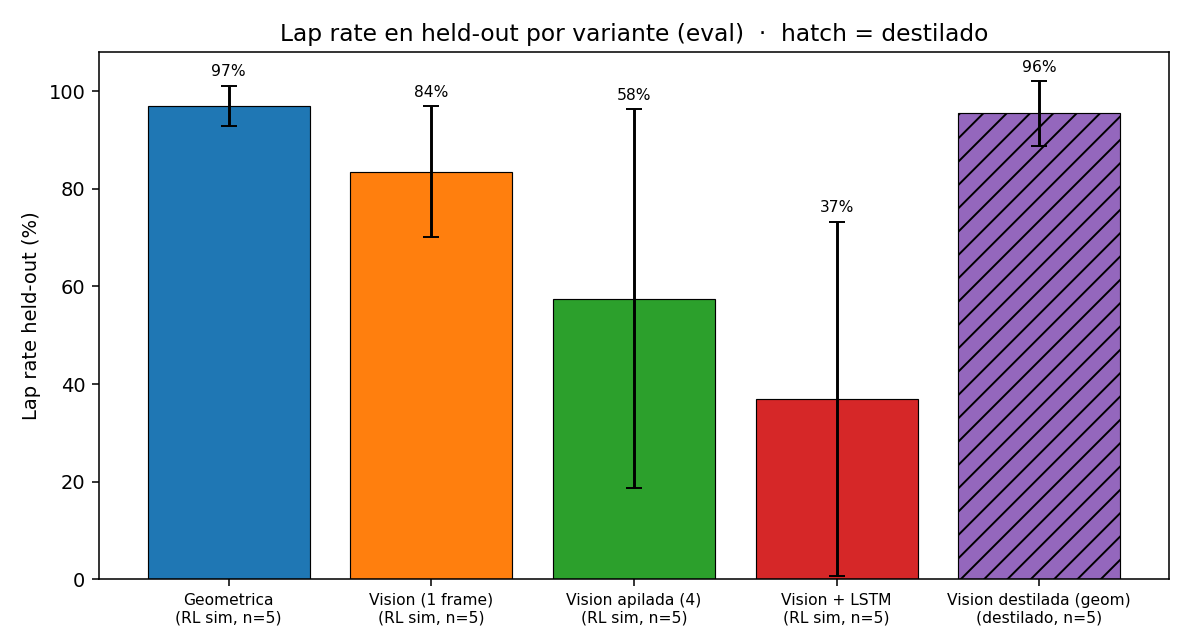
\includegraphics[width=\linewidth]{figures/fig_eval_lap_rate.png}
\caption{Lap rate en pistas no vistas por variante ($5$ semillas, fondo aleatorio). La
geom\'etrica y la destilada quedan arriba y con barras angostas; la visi\'on-RL cae y, sobre
todo, se vuelve \emph{inestable}.}
\label{fig:eval}
\end{figure}

El hallazgo central: la \textbf{visi\'on destilada es estad\'isticamente indistinguible del
maestro privilegiado} (Tabla~\ref{tab:sig}, $p = 1.000$ por Mann-Whitney exacto de dos colas
sobre $5$ semillas), y adem\'as es el \emph{conductor confiable m\'as r\'apido}: recupera la
competencia del agente privilegiado partiendo solo de p\'ixeles.

\subsection{La visi\'on-RL es una loter\'ia; la destilaci\'on, no}
El promedio esconde lo esencial. La Tabla~\ref{tab:seed} muestra el lap rate por semilla: las
variantes temporales son \textbf{bimodales} ---algunas semillas convergen y otras colapsan
(de $5$ a $100$, de $0$ a $82$)--- mientras que el maestro y la destilada rinden parejo en las
cinco. La enorme varianza de apilada y LSTM es el s\'intoma: la temporalidad agrega
\emph{dificultad de optimizaci\'on}, no desempe\~no. Diagn\'osticos de entrenamiento
(divergencia de KL, \emph{explained variance} negativa del cr\'itico) confirman una
optimizaci\'on inestable.

\begin{table}[t]
\caption{Lap rate (\%) por semilla. Verde $\geq 85$, rojo $< 50$.}
\label{tab:seed}
\centering
\small
\begin{tabular}{@{}lrrrrr@{}}
\toprule
\textbf{Variante} & \textbf{s0} & \textbf{s1} & \textbf{s2} & \textbf{s3} & \textbf{s4} \\
\midrule
Geom\'etrica       & \cellcolor{goodbg}100 & \cellcolor{goodbg}98 & \cellcolor{goodbg}98 & \cellcolor{goodbg}90 & \cellcolor{goodbg}100 \\
Visi\'on destilada & \cellcolor{goodbg}100 & \cellcolor{goodbg}92 & \cellcolor{goodbg}100 & \cellcolor{goodbg}100 & \cellcolor{goodbg}85 \\
Visi\'on 1 cuadro  & \cellcolor{goodbg}90 & \cellcolor{goodbg}92 & 60 & \cellcolor{goodbg}90 & \cellcolor{goodbg}85 \\
Visi\'on apilada   & \cellcolor{badbg}38 & \cellcolor{goodbg}90 & \cellcolor{badbg}5 & 55 & \cellcolor{goodbg}100 \\
Visi\'on + LSTM    & \cellcolor{badbg}5 & 65 & \cellcolor{badbg}0 & \cellcolor{badbg}32 & 82 \\
\bottomrule
\end{tabular}
\end{table}

\begin{table}[t]
\caption{Significancia (Mann-Whitney exacto, dos colas, sobre lap rate por semilla, $n{=}5$).
$^{*}\,p<0.05$; $^{**}\,p<0.01$; n.s.\ = no significativo.}
\label{tab:sig}
\centering
\small
\begin{tabular}{@{}lrl@{}}
\toprule
\textbf{Comparaci\'on} & \textbf{$p$} & \textbf{Veredicto} \\
\midrule
\rowcolor{goodbg} Geom\'etrica vs Destilada       & $1.000$ & sin diferencia \\
Geom\'etrica vs 1 cuadro          & $0.032$ & $^{*}$ \\
Geom\'etrica vs LSTM              & $0.008$ & $^{**}$ \\
Destilada vs LSTM                 & $0.008$ & $^{**}$ \\
Destilada vs 1 cuadro             & $0.079$ & marginal \\
1 cuadro vs LSTM                  & $0.032$ & $^{*}$ \\
Destilada vs apilada              & $0.103$ & n.s. \\
Geom\'etrica vs apilada           & $0.127$ & n.s. \\
\bottomrule
\end{tabular}
\end{table}

\section{An\'alisis: qu\'e mira la CNN}
Para entender \emph{por qu\'e} la destilaci\'on funciona, calculamos saliencia por
\emph{guided backprop}~\cite{springenberg2015guided}: el gradiente de la decisi\'on (valor del
cr\'itico $V(s)$ y \emph{steering}) respecto de los p\'ixeles de entrada. Crucialmente, la
saliencia se computa \textbf{sobre el mismo cuadro que se muestra} ---una curva--- y no como un
promedio sobre cuadros distintos, que mezclar\'ia rectas y curvas. La Fig.~\ref{fig:saliency}
compara las cuatro variantes de visi\'on (todas semilla $0$).

\begin{figure*}[t]
\centering
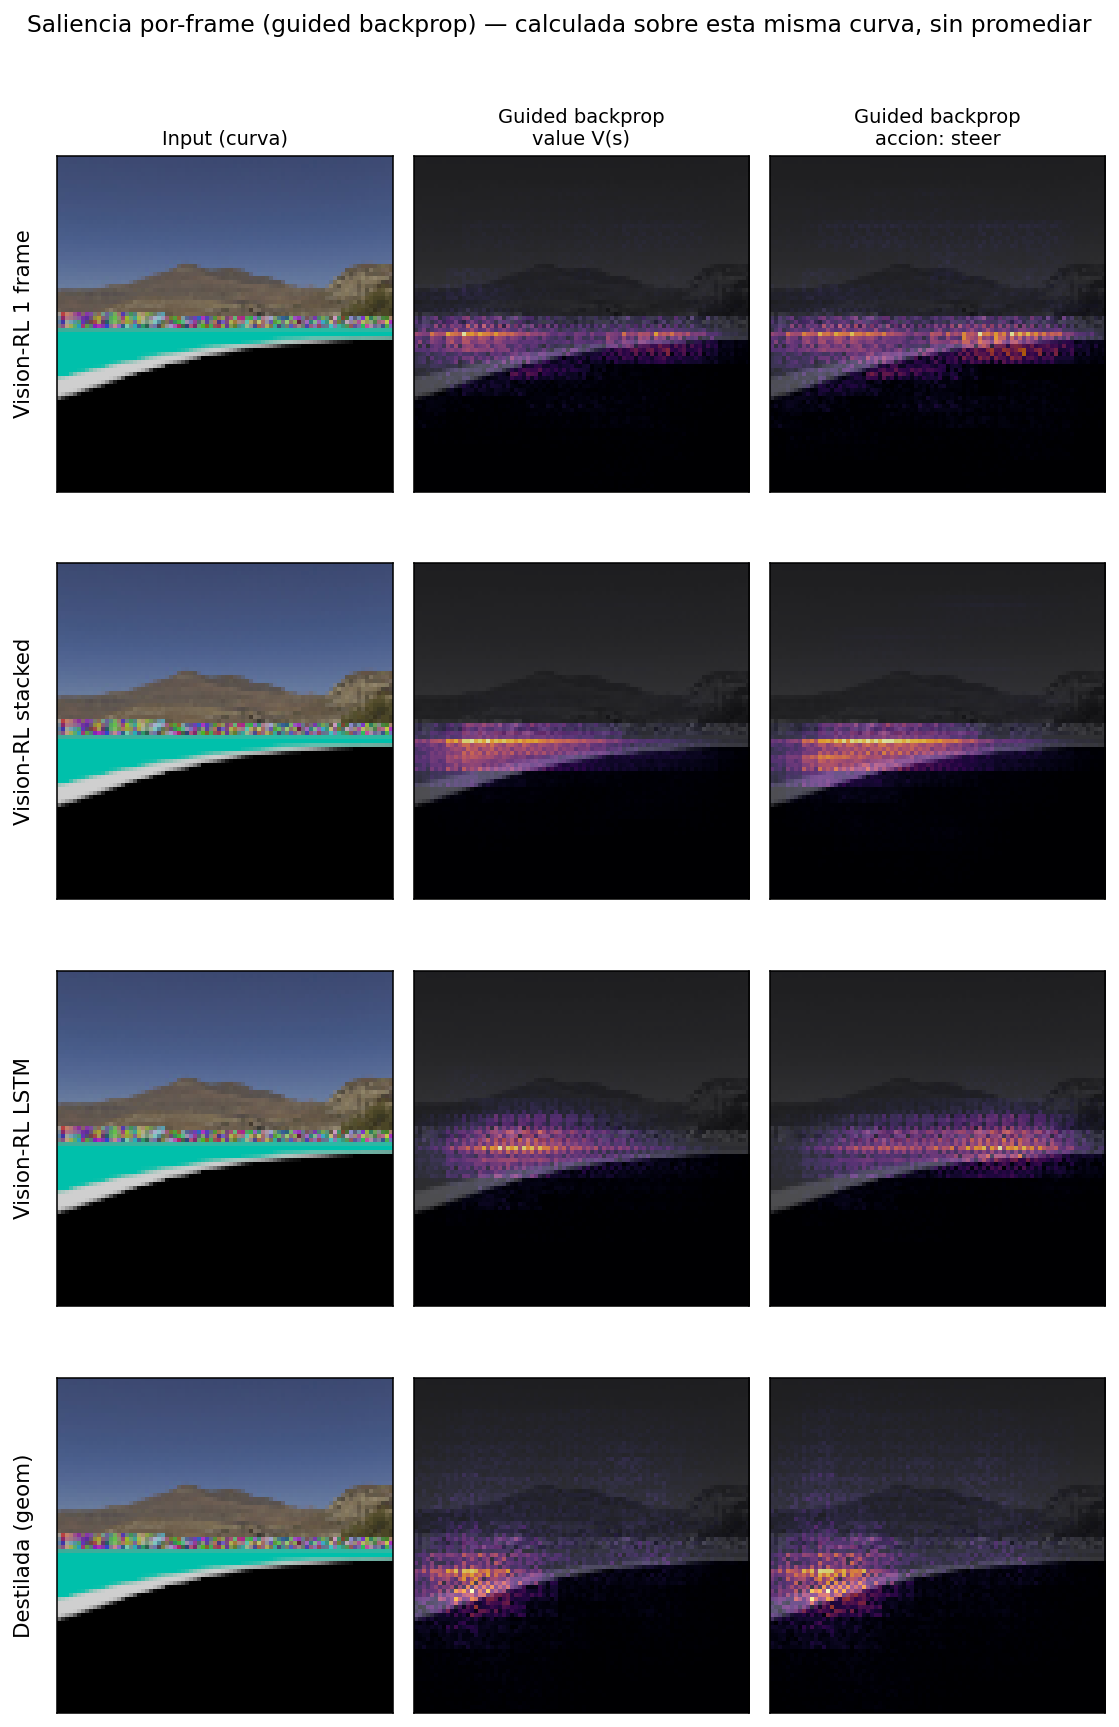
\includegraphics[width=0.72\textwidth]{figures/fig_saliency.png}
\caption{Saliencia por \emph{guided backprop} sobre una misma curva. Las tres variantes
RL puras (1 cuadro, apilada, LSTM) encienden la saliencia en una franja sobre el
\textbf{horizonte} ---la pared y las monta\~nas del fondo---: usan el entorno, constante en
entrenamiento, como atajo. La \textbf{destilada} desplaza la atenci\'on hacia \emph{abajo},
sobre la calzada y el borde curvo del carril, con el horizonte apagado: hereda del maestro
geom\'etrico \emph{qu\'e mirar}. Dentro de cada modelo, \emph{value} y \emph{steer} coinciden
porque comparten el extractor CNN.}
\label{fig:saliency}
\end{figure*}

La lectura es directa: la visi\'on-RL directa se apoya en el fondo, que correlaciona con la
direcci\'on del giro en el set de entrenamiento pero desaparece bajo randomizaci\'on; la
destilaci\'on \emph{decorrelaciona} la pol\'itica del fondo, y por eso se sostiene. La
Fig.~\ref{fig:curves} muestra adem\'as que la visi\'on-RL aprende m\'as lento y con bandas
m\'as anchas que el maestro.

\begin{figure}[t]
\centering

\includegraphics[width=0.49\linewidth]{figures/fig_reward.png}\hfill

\includegraphics[width=0.49\linewidth]{figures/fig_lap_rate.png}
\caption{Curvas de entrenamiento de las variantes RL ($5$ semillas, banda $=\pm$ desv\'io).
Izquierda: reward por episodio. Derecha: lap rate en pistas no vistas durante el entrenamiento.
La destilada es supervisada y no aparece en estas curvas de RL.}
\label{fig:curves}
\end{figure}

\section{Limitaciones}
El estudio es \textbf{solo en simulaci\'on}: no evaluamos transferencia a hardware real, y el
maestro usa features extra\'idas dentro del simulador que en el mundo real habr\'ia que estimar
con percepci\'on ---el problema dif\'icil. La \textbf{familia de pistas es acotada} (dos pistas
no vistas de la misma distribuci\'on) y la \textbf{randomizaci\'on de dominio es parcial}
(var\'ia pared y skybox, no geometr\'ia, iluminaci\'on ni c\'amara), de modo que cierra
\emph{este} atajo y no todos los posibles. Por construcci\'on, el \textbf{estudiante hereda el
techo del maestro}: la mejora en tiempo de vuelta proviene de acciones m\'as suaves, no de una
pol\'itica estrictamente superior. Finalmente, la bimodalidad de la visi\'on-RL sugiere alta
\textbf{sensibilidad a la semilla}; no realizamos un barrido exhaustivo que pudiera rescatar
algunas semillas colapsadas.

\section{Conclusi\'on}
Un agente privilegiado con percepci\'on limpia de la calzada resuelve la tarea ($97\%$), y
\emph{destilarlo} a visi\'on pura recupera ese desempe\~no sin p\'erdida significativa
($95.5\%$, $p = 1.0$) y con mejor tiempo de vuelta. Entrenar la misma visi\'on con RL directo es
poco confiable, y la temporalidad la empeora. La randomizaci\'on del fondo y la saliencia
confirman que la ventaja es de \emph{invarianza al entorno}: la destilada mira la calzada, no el
horizonte. La lectura general es que el l\'imite de la visi\'on-RL no es la \emph{capacidad} de
la representaci\'on sino la \emph{asignaci\'on de cr\'edito} a trav\'es de p\'ixeles en un
problema parcialmente observable; la destilaci\'on privilegiada lo esquiva con targets
supervisados densos del agente privilegiado. C\'odigo, modelos y una versi\'on navegable del
paper est\'an disponibles en \url{https://github.com/fluchetti45/deepracer}.

\FloatBarrier
\bibliographystyle{IEEEtran}
\bibliography{references}

\end{document}
